\documentclass[11pt,a4paper,fontset=fandol]{ctexart}

\usepackage[a4paper,top=2.45cm,bottom=2.6cm,left=2.35cm,right=2.35cm,headheight=18pt,headsep=0.55cm,footskip=26pt]{geometry}
\usepackage{amsmath,amssymb,amsthm}
\usepackage{fancyhdr}
\usepackage{lastpage}
\usepackage{enumitem}
\usepackage{titlesec}
\usepackage{xcolor}
\usepackage{tikz}
\usepackage{hyperref}
\usepackage{bookmark}
\usepackage[most]{tcolorbox}
\usepackage{setspace}
\usepackage{array}
\usetikzlibrary{arrows.meta,positioning}

\hypersetup{
  colorlinks=true,
  linkcolor=blue!50!black,
  urlcolor=blue!50!black,
  citecolor=blue!50!black
}

\setstretch{1.17}
\setlength{\parindent}{2em}
\setlength{\parskip}{0.35em}
\allowdisplaybreaks
\setlist[enumerate]{itemsep=0.32em, topsep=0.32em, leftmargin=2.3em}
\setlist[itemize]{itemsep=0.25em, topsep=0.25em, leftmargin=2em}
\setcounter{tocdepth}{2}

\definecolor{mainblue}{RGB}{36,83,140}
\definecolor{lightblue}{RGB}{241,246,252}
\definecolor{lightgray}{RGB}{246,246,246}
\definecolor{accent}{RGB}{153,76,0}
\definecolor{rulegray}{RGB}{110,118,128}
\definecolor{softgreen}{RGB}{236,247,240}

\titleformat{\section}
  {\Large\bfseries\color{mainblue}}
  {\thesection.}
  {0.45em}
  {}
  [\vspace{0.25em}\color{rulegray}\titlerule]
\titlespacing*{\section}{0pt}{1.3em}{0.9em}
\titleformat{\subsection}{\large\bfseries\color{mainblue}}{\thesubsection}{0.5em}{}
\titlespacing*{\subsection}{0pt}{1.05em}{0.55em}
\titleformat{\subsubsection}{\normalsize\bfseries\color{accent}}{\thesubsubsection}{0.5em}{}

\pagestyle{fancy}
\fancyhf{}
\fancyhead[L]{\small 代数专题课堂讲义}
\fancyhead[C]{\small 函数图像平移与方程}
\fancyhead[R]{\small 刘文博}
\fancyfoot[C]{\small 第 \thepage 页 / 共 \pageref{LastPage} 页}
\renewcommand{\headrulewidth}{0.55pt}
\renewcommand{\footrulewidth}{0.35pt}

\newtheoremstyle{formaltheorem}
  {0.8em}{0.8em}{\normalfont}{}{\bfseries\color{mainblue}}{．}{0.6em}{}
\newtheoremstyle{formalexample}
  {0.8em}{0.8em}{\normalfont}{}{\bfseries\color{accent}}{．}{0.6em}{}

\theoremstyle{formaltheorem}
\newtheorem{theorem}{结论}[section]
\newtheorem{method}{方法}[section]
\theoremstyle{formalexample}
\newtheorem{example}{例题}[section]
\newtheorem{exercise}{练习}[section]

\newenvironment{solution}{\par\noindent\textbf{解：}}{\hfill$\square$\par}

\newtcolorbox{goalbox}[1]{
  breakable,
  colback=lightblue,
  colframe=mainblue,
  boxrule=0.7pt,
  arc=1mm,
  left=1.2mm,
  right=1.2mm,
  top=1mm,
  bottom=1mm,
  title=\textbf{#1},
  fonttitle=\bfseries
}

\newtcolorbox{notebox}[1]{
  breakable,
  colback=lightgray,
  colframe=black!50,
  boxrule=0.55pt,
  arc=1mm,
  left=1.2mm,
  right=1.2mm,
  top=1mm,
  bottom=1mm,
  title=\textbf{#1},
  fonttitle=\bfseries
}

\newtcolorbox{skillbox}[1]{
  breakable,
  colback=softgreen,
  colframe=green!40!black,
  boxrule=0.65pt,
  arc=1mm,
  left=1.2mm,
  right=1.2mm,
  top=1mm,
  bottom=1mm,
  title=\textbf{#1},
  fonttitle=\bfseries
}

\newcommand{\basef}{y=f(x)}

\begin{document}

\thispagestyle{empty}
\begin{titlepage}
\centering
\vspace*{0.9cm}

\begin{tcolorbox}[
  enhanced,
  width=0.92\textwidth,
  colback=white,
  colframe=mainblue,
  boxrule=1pt,
  arc=0mm,
  left=6mm,
  right=6mm,
  top=8mm,
  bottom=8mm
]
\centering

{\fontsize{24}{30}\selectfont\bfseries 代数专题课堂讲义\par}
\vspace{0.7cm}
{\fontsize{17}{22}\selectfont 函数图像平移与方程\par}

\vspace{1.1cm}
\color{rulegray}\rule{0.72\textwidth}{0.7pt}\par
\vspace{1cm}

\begin{tcolorbox}[colback=lightblue,colframe=mainblue,width=0.82\textwidth,boxrule=1pt]
\centering
{\Large 适合对象：初中阶段正在学习函数的学生}\\[0.4em]
{\large 已学过坐标系、一次函数、二次函数或基本函数图像}
\end{tcolorbox}

\vspace{1.2cm}

\renewcommand{\arraystretch}{1.42}
\begin{tabular}{>{\bfseries}p{3.5cm}p{8cm}}
讲义作者： & 刘文博 \\
专题关键词： & 图像平移、方程变形、向上、向下、向左、向右 \\
建议课时： & 1--2 课时 \\
专题目标： & 学会从已知函数方程快速写出平移后的新方程，并能反向判断平移方向 \\
编译方式： & XeLaTeX \\
\end{tabular}

\vspace{1.2cm}
\color{rulegray}\rule{0.72\textwidth}{0.7pt}\par
\vspace{0.8cm}

{\normalsize 本讲以“图像怎么动，方程怎么改”为主线，重点解决学生最容易混淆的左右平移符号问题，并配上可直接订正的练习。\par}

\vspace{0.5cm}
{\large \today\par}
\end{tcolorbox}
\end{titlepage}

\pagenumbering{Roman}
\pagestyle{plain}
\tableofcontents
\newpage
\pagestyle{fancy}
\pagenumbering{arabic}

\section{专题目标与使用说明}

\begin{goalbox}{本讲要解决的核心问题}
已知一个函数的方程，例如
\[
y=f(x),
\]
如果把它的图像向上、向下、向左、向右平移，新的函数方程该怎么写？

这是初中函数学习里非常重要的一步，因为它把\textbf{图像变化}和\textbf{代数式变化}连在了一起。
\end{goalbox}

\begin{goalbox}{学完以后希望达到的能力}
\begin{itemize}
  \item 看见“向上平移 $k$ 个单位”就能立即写出 $y=f(x)+k$；
  \item 看见“向下平移 $k$ 个单位”就能立即写出 $y=f(x)-k$；
  \item 看见“向左平移 $a$ 个单位”就能立即写出 $y=f(x+a)$；
  \item 看见“向右平移 $a$ 个单位”就能立即写出 $y=f(x-a)$；
  \item 会处理既有左右平移、又有上下平移的综合题；
  \item 能反向从新方程判断原图像是怎样平移得到的。
\end{itemize}
\end{goalbox}

\begin{notebox}{给家长和自学同学的提醒}
\begin{itemize}
  \item 本讲的最大难点不在计算，而在\textbf{左右平移的符号容易写反}；
  \item 建议每做一道题，都先口头说一遍：“这是图像向哪边走，不是式子里的字母往哪边改”；
  \item 真正掌握的标准不是背公式，而是能用“关键点跟着移动”去验证。
\end{itemize}
\end{notebox}

\section{先抓住最根本的图像变化}

\subsection{把图像当作很多点的集合}
函数图像可以看成许多点组成的集合。如果点 $(x_0,y_0)$ 在图像 $\basef$ 上，那么一定有
\[
y_0=f(x_0).
\]
因此，研究图像平移时，最自然的方法就是研究：\textbf{图上的每一个点平移以后，新坐标变成什么。}

\begin{method}
若原图像上有点 $(x_0,y_0)$，那么：
\begin{itemize}
  \item 向上平移 $k$ 个单位后，它变成 $(x_0,y_0+k)$；
  \item 向下平移 $k$ 个单位后，它变成 $(x_0,y_0-k)$；
  \item 向右平移 $a$ 个单位后，它变成 $(x_0+a,y_0)$；
  \item 向左平移 $a$ 个单位后，它变成 $(x_0-a,y_0)$。
\end{itemize}
\end{method}

\subsection{竖直平移比水平平移更直观}
如果整张图像向上或向下移动，那么每个点的横坐标都不变，只是纵坐标一起增加或减少。

所以竖直平移时，改变的是函数值，也就是\textbf{$y$ 这一侧}。

如果整张图像向左或向右移动，那么每个点的纵坐标不变，只是横坐标一起变化。

所以水平平移时，真正改变的是“哪个 $x$ 对应到这个函数值”，也就是\textbf{$x$ 这一侧}。

\section{四种基本平移公式}

\subsection{向上、向下平移}

\begin{theorem}
已知原函数为
\[
y=f(x).
\]
\begin{itemize}
  \item 向上平移 $k$ 个单位（$k>0$），所得新方程为
  \[
  y=f(x)+k;
  \]
  \item 向下平移 $k$ 个单位（$k>0$），所得新方程为
  \[
  y=f(x)-k.
  \]
\end{itemize}
\end{theorem}

\begin{solution}
竖直平移时，每个点的横坐标不变，纵坐标统一加上或减去 $k$。所以函数值整体变大或变小，自然表现为在原式外面加 $k$ 或减 $k$。
\end{solution}

\subsection{向左、向右平移}

\begin{theorem}
已知原函数为
\[
y=f(x).
\]
\begin{itemize}
  \item 向左平移 $a$ 个单位（$a>0$），所得新方程为
  \[
  y=f(x+a);
  \]
  \item 向右平移 $a$ 个单位（$a>0$），所得新方程为
  \[
  y=f(x-a).
  \]
\end{itemize}
\end{theorem}

\begin{solution}
这部分最容易混淆。以向右平移 $a$ 个单位为例：

原图像上点 $(x_0,y_0)$ 平移后变成 $(x_0+a,y_0)$。设新图像上的横坐标记成 $x$，那么它对应原图像上的横坐标就是 $x-a$，因此新函数值应为
\[
y=f(x-a).
\]
同理，向左平移 $a$ 个单位后应写成
\[
y=f(x+a).
\]
\end{solution}

\begin{skillbox}{一句话记忆}
\begin{itemize}
  \item 上下平移：\textbf{在函数外面加减}；
  \item 左右平移：\textbf{在函数里面改 $x$}；
  \item 左加右减：\textbf{图像向左，式子里加；图像向右，式子里减。}
\end{itemize}
\end{skillbox}

\subsection{图像直观对比}

\begin{center}
\begin{minipage}{0.48\textwidth}
\centering
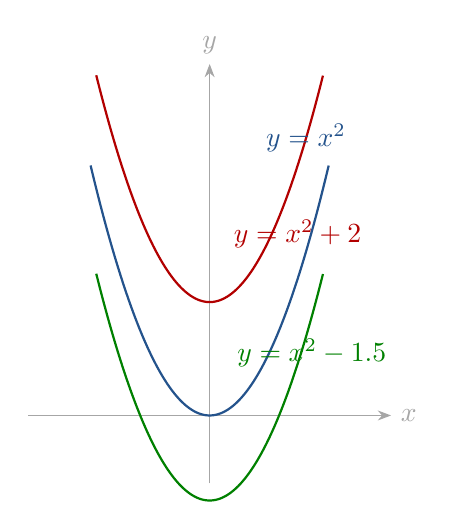
\begin{tikzpicture}[scale=0.72,>=Stealth]
  \draw[->,gray!70] (-3.2,0) -- (3.2,0) node[right] {$x$};
  \draw[->,gray!70] (0,-1.2) -- (0,6.2) node[above] {$y$};
  \draw[smooth,domain=-2.1:2.1,samples=100,thick,mainblue] plot (\x,{(\x)*(\x)});
  \draw[smooth,domain=-2:2,samples=100,thick,red!70!black] plot (\x,{(\x)*(\x)+2});
  \draw[smooth,domain=-2:2,samples=100,thick,green!50!black] plot (\x,{(\x)*(\x)-1.5});
  \node[mainblue] at (1.7,4.9) {$y=x^2$};
  \node[red!70!black] at (1.55,3.2) {$y=x^2+2$};
  \node[green!50!black] at (1.8,1.1) {$y=x^2-1.5$};
\end{tikzpicture}

\small 竖直平移：在函数外面加减
\end{minipage}
\hfill
\begin{minipage}{0.48\textwidth}
\centering
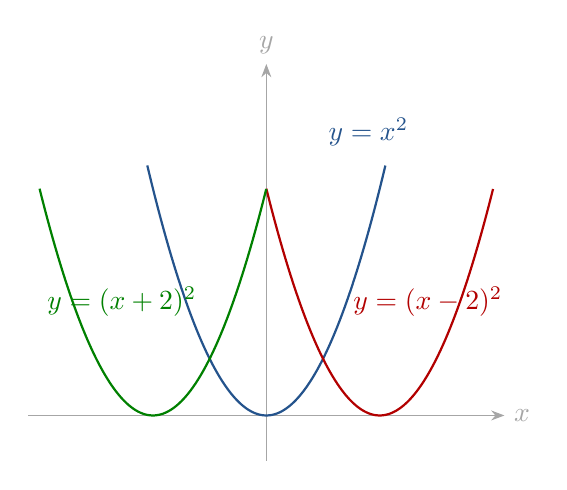
\begin{tikzpicture}[scale=0.72,>=Stealth]
  \draw[->,gray!70] (-4.2,0) -- (4.2,0) node[right] {$x$};
  \draw[->,gray!70] (0,-0.8) -- (0,6.2) node[above] {$y$};
  \draw[smooth,domain=-2.1:2.1,samples=100,thick,mainblue] plot (\x,{(\x)*(\x)});
  \draw[smooth,domain=0:4,samples=100,thick,red!70!black] plot (\x,{(\x-2)*(\x-2)});
  \draw[smooth,domain=-4:0,samples=100,thick,green!50!black] plot (\x,{(\x+2)*(\x+2)});
  \node[mainblue] at (1.8,5) {$y=x^2$};
  \node[red!70!black] at (2.85,2.0) {$y=(x-2)^2$};
  \node[green!50!black] at (-2.55,2.0) {$y=(x+2)^2$};
\end{tikzpicture}

\small 水平平移：在函数里面改 $x$
\end{minipage}
\end{center}

\section{求平移后方程的两种常用方法}

\subsection{方法一：直接套公式}
当题目已经明确告诉你平移方向和距离时，最直接的方法就是使用四个基本公式。

\begin{method}
若原函数为 $\basef$，则：
\[
\begin{array}{rcl}
\text{向上平移 }k\text{ 个单位} &\Longrightarrow& y=f(x)+k,\\[0.4em]
\text{向下平移 }k\text{ 个单位} &\Longrightarrow& y=f(x)-k,\\[0.4em]
\text{向左平移 }a\text{ 个单位} &\Longrightarrow& y=f(x+a),\\[0.4em]
\text{向右平移 }a\text{ 个单位} &\Longrightarrow& y=f(x-a).
\end{array}
\]
\end{method}

\begin{example}
把抛物线
\[
y=x^2
\]
向右平移 $2$ 个单位，再向上平移 $3$ 个单位，求新方程。
\end{example}

\begin{solution}
先向右平移 $2$ 个单位，得到
\[
y=(x-2)^2.
\]
再向上平移 $3$ 个单位，得到
\[
y=(x-2)^2+3.
\]
所以新方程是
\[
\boxed{y=(x-2)^2+3}.
\]
\end{solution}

\subsection{方法二：抓关键点验证}
如果担心公式写反，可以抓住图像上的关键点，比如：
\begin{itemize}
  \item 一次函数上的截距点；
  \item 二次函数上的顶点；
  \item 绝对值函数的尖点；
  \item 反比例函数上的特殊点。
\end{itemize}
关键点跟着平移后，新方程必须把这些点包含进去。

\begin{example}
已知函数
\[
y=|x|
\]
向左平移 $1$ 个单位，再向下平移 $2$ 个单位，求新方程。
\end{example}

\begin{solution}
原图像的关键点是顶点 $(0,0)$。

向左平移 $1$ 个单位后，顶点到 $( -1,0 )$；

再向下平移 $2$ 个单位后，顶点到 $( -1,-2 )$。

因此新图像应当是一个顶点在 $( -1,-2 )$ 的“V”形图像，所以方程应为
\[
y=|x+1|-2.
\]

检验一下：当 $x=-1$ 时，
\[
y=|-1+1|-2=-2,
\]
正好得到顶点 $( -1,-2 )$，说明结果正确。
\end{solution}

\section{综合平移时怎样一步写出结果}

\subsection{统一写法}
如果把 $\basef$ 先左右平移，再上下平移，最终都可以统一写成
\[
y=f(x-a)+b.
\]
这里：
\begin{itemize}
  \item $a>0$ 表示向右平移 $a$ 个单位；
  \item $a<0$ 表示向左平移 $|a|$ 个单位；
  \item $b>0$ 表示向上平移 $b$ 个单位；
  \item $b<0$ 表示向下平移 $|b|$ 个单位。
\end{itemize}

\begin{skillbox}{统一判断口诀}
\[
y=f(x-a)+b
\]
表示“\textbf{右 $a$ 上 $b$}”。

如果看到
\[
y=f(x+3)-2,
\]
就把它看成
\[
y=f(x-(-3))+(-2),
\]
于是图像是\textbf{向左平移 $3$ 个单位，再向下平移 $2$ 个单位}。
\end{skillbox}

\subsection{两个典型例题}

\begin{example}
把直线
\[
y=2x-1
\]
向左平移 $4$ 个单位，再向下平移 $5$ 个单位，求新方程。
\end{example}

\begin{solution}
向左平移 $4$ 个单位，应把 $x$ 换成 $x+4$，得到
\[
y=2(x+4)-1.
\]
再向下平移 $5$ 个单位，得到
\[
y=2(x+4)-1-5.
\]
化简得
\[
y=2x+2.
\]
所以新方程是
\[
\boxed{y=2x+2}.
\]
\end{solution}

\begin{example}
把函数
\[
y=x^2-4x+1
\]
向右平移 $1$ 个单位，再向上平移 $2$ 个单位，求新方程。
\end{example}

\begin{solution}
先做右平移：把式子里的 $x$ 换成 $x-1$，得
\[
y=(x-1)^2-4(x-1)+1.
\]
再向上平移 $2$ 个单位，得
\[
y=(x-1)^2-4(x-1)+3.
\]
化简：
\[
y=x^2-6x+8.
\]
所以新方程是
\[
\boxed{y=x^2-6x+8}.
\]
\end{solution}

\section{最容易犯的几个错误}

\begin{notebox}{误区一：把左右平移的符号写反}
很多同学看到“向右平移 $3$ 个单位”，就误写成
\[
y=f(x+3).
\]
这是错误的。正确写法是
\[
y=f(x-3).
\]
因为图像向右走，式子里要减。
\end{notebox}

\begin{notebox}{误区二：只改一部分，不改整个 $x$}
例如原函数是
\[
y=x^2-4x+1.
\]
如果向右平移 $2$ 个单位，不能只把前面的 $x^2$ 改成 $(x-2)^2$，后面的 $-4x$ 还不动。

正确做法是把\textbf{整个式子里的 $x$ 都替换成 $x-2$}，即
\[
y=(x-2)^2-4(x-2)+1.
\]
\end{notebox}

\begin{notebox}{误区三：只会背公式，不会检验}
如果你算出了一个新方程，一定要拿关键点检验一下。比如原图像顶点是 $(0,0)$，向右平移 $2$ 个单位后，顶点应该变成 $(2,0)$。如果你的方程代入 $x=2$ 却得不到 $y=0$，说明式子写错了。
\end{notebox}

\section{例题讲解}

\begin{example}
已知函数
\[
y=3x+2,
\]
将它的图像向右平移 $1$ 个单位，再向下平移 $4$ 个单位，求新方程。
\end{example}

\begin{solution}
先向右平移 $1$ 个单位：
\[
y=3(x-1)+2.
\]
再向下平移 $4$ 个单位：
\[
y=3(x-1)+2-4.
\]
化简得
\[
y=3x-5.
\]
所以新方程是
\[
\boxed{y=3x-5}.
\]
\end{solution}

\begin{example}
已知抛物线
\[
y=x^2
\]
经过平移后变为
\[
y=(x+2)^2-5.
\]
求它是由原图像怎样平移得到的。
\end{example}

\begin{solution}
把新方程和统一形式
\[
y=f(x-a)+b
\]
对照。

这里
\[
y=(x+2)^2-5=(x-(-2))^2+(-5).
\]
所以 $a=-2$，$b=-5$。

这说明原图像是\textbf{向左平移 $2$ 个单位，再向下平移 $5$ 个单位}得到的。
\end{solution}

\begin{example}
已知函数
\[
y=|x-3|+1.
\]
求它是由
\[
y=|x|
\]
怎样平移得到的。
\end{example}

\begin{solution}
与
\[
y=f(x-a)+b
\]
比较可知，这里 $a=3$，$b=1$。

因此图像是由 $y=|x|$ \textbf{向右平移 $3$ 个单位，再向上平移 $1$ 个单位}得到的。

也可以从顶点看：$y=|x|$ 的顶点是 $(0,0)$，而 $y=|x-3|+1$ 的顶点是 $(3,1)$，完全一致。
\end{solution}

\section{课堂练习}

\begin{exercise}
把函数
\[
y=x^2
\]
向上平移 $4$ 个单位，写出新方程。
\end{exercise}

\begin{exercise}
把函数
\[
y=x^2
\]
向左平移 $3$ 个单位，写出新方程。
\end{exercise}

\begin{exercise}
把函数
\[
y=2x+1
\]
向右平移 $2$ 个单位，再向上平移 $5$ 个单位，写出新方程。
\end{exercise}

\begin{exercise}
把函数
\[
y=|x|
\]
向右平移 $4$ 个单位，再向下平移 $1$ 个单位，写出新方程。
\end{exercise}

\begin{exercise}
已知函数
\[
y=(x-5)^2+2,
\]
说出它是由
\[
y=x^2
\]
怎样平移得到的。
\end{exercise}

\begin{exercise}
已知函数
\[
y=3(x+1)-4,
\]
说出它是由
\[
y=3x
\]
怎样平移得到的。
\end{exercise}

\begin{exercise}
把函数
\[
y=x^2+2x
\]
向左平移 $1$ 个单位，再向下平移 $3$ 个单位，写出新方程。
\end{exercise}

\begin{exercise}
已知函数
\[
y=f(x)
\]
经过平移后变为
\[
y=f(x+6)-7.
\]
说出它是怎样平移得到的。
\end{exercise}

\section{练习解答}

\begin{solution}
\textbf{第 1 题：}
向上平移 $4$ 个单位，就是在原式外面加 $4$，所以
\[
\boxed{y=x^2+4}.
\]
\end{solution}

\begin{solution}
\textbf{第 2 题：}
向左平移 $3$ 个单位，就是把 $x$ 换成 $x+3$，所以
\[
\boxed{y=(x+3)^2}.
\]
\end{solution}

\begin{solution}
\textbf{第 3 题：}
先向右平移 $2$ 个单位，得
\[
y=2(x-2)+1.
\]
再向上平移 $5$ 个单位，得
\[
y=2(x-2)+1+5=2x+2.
\]
所以
\[
\boxed{y=2x+2}.
\]
\end{solution}

\begin{solution}
\textbf{第 4 题：}
向右平移 $4$ 个单位，得到
\[
y=|x-4|.
\]
再向下平移 $1$ 个单位，得到
\[
\boxed{y=|x-4|-1}.
\]
\end{solution}

\begin{solution}
\textbf{第 5 题：}
\[
y=(x-5)^2+2
\]
表示在 $y=x^2$ 的基础上，先向右平移 $5$ 个单位，再向上平移 $2$ 个单位。
\end{solution}

\begin{solution}
\textbf{第 6 题：}
先把式子整理成
\[
y=3x+3-4=3x-1.
\]
但题目是让我们从
\[
y=3x
\]
来观察平移关系，更直接的看法是：
\[
y=3(x+1)-4
\]
表示先向左平移 $1$ 个单位，再向下平移 $4$ 个单位。
\end{solution}

\begin{solution}
\textbf{第 7 题：}
向左平移 $1$ 个单位，应把整个式子里的 $x$ 都换成 $x+1$，得
\[
y=(x+1)^2+2(x+1).
\]
再向下平移 $3$ 个单位，得
\[
y=(x+1)^2+2(x+1)-3.
\]
化简：
\[
y=x^2+4x.
\]
所以
\[
\boxed{y=x^2+4x}.
\]
\end{solution}

\begin{solution}
\textbf{第 8 题：}
\[
y=f(x+6)-7=f(x-(-6))+(-7).
\]
因此图像是由原图像\textbf{向左平移 $6$ 个单位，再向下平移 $7$ 个单位}得到的。
\end{solution}

\section{本讲小结}

\begin{goalbox}{四个最关键的结论}
\[
\begin{array}{rcl}
\text{向上 }k\text{ 个单位} &\Longrightarrow& y=f(x)+k,\\[0.4em]
\text{向下 }k\text{ 个单位} &\Longrightarrow& y=f(x)-k,\\[0.4em]
\text{向左 }a\text{ 个单位} &\Longrightarrow& y=f(x+a),\\[0.4em]
\text{向右 }a\text{ 个单位} &\Longrightarrow& y=f(x-a).
\end{array}
\]
\end{goalbox}

\begin{skillbox}{最后再提醒一次}
\begin{itemize}
  \item 上下平移看“外面”；
  \item 左右平移看“里面”；
  \item 左加右减最容易错，必须反复检查；
  \item 遇到综合题，统一看成
  \[
  y=f(x-a)+b.
  \]
\end{itemize}
\end{skillbox}

\begin{notebox}{自检清单}
\begin{itemize}
  \item 我能不能不看答案，直接写出 $y=|x|$ 向左 $2$、向上 $3$ 后的方程？
  \item 我能不能解释为什么“向右平移”反而要写成 $x-a$？
  \item 我会不会用顶点、截距点等关键点做检验？
\end{itemize}
如果这三项都能做到，就说明这部分已经真正掌握了。
\end{notebox}

\end{document}
